\section{Results}

\subsection{Results on Iterative Characteristics and Hulls}

We apply our algorithms in Section \ref{sec:find_ite_c} and \ref{sec:find_ite_h} to some PRESENT-like ciphers having a 

\subsubsection{RECTANGLE} We set $A=2,3$ and the equivalance relation to be $=_R$. 

\subsubsection{PRESENT} We set $A=2,3$

\subsubsection{GIFT}

\subsubsection{PUFFIN,EPCBC,TRIFLE} PUFFIN, EPCBC, TRIFLE-BC are another three PRESENT-like block ciphers. 

\begin{figure}\label{fig:plot_ite}
    \centering
    \caption{Results on some SPN block ciphers, which are RECTANGLE, PRESENT, GIFT64, PUFFIN, EPCBC and TRIFLE from top to bottom resp. For each subfigure, the x-axis is the number of rounds. For a subfigure in the left column, the y-axis is the weight of differential probability, while for a subfigure in the right column, the y-axis is the weight of correlation square. The red spot denotes the best single iterative characteristic with fewest rounds obtained by Algo. \ref{algo:find_ite_c_G}. The yellow (green, blue) line denotes the best iterative hull with $A=$1 (2, 3).} 
	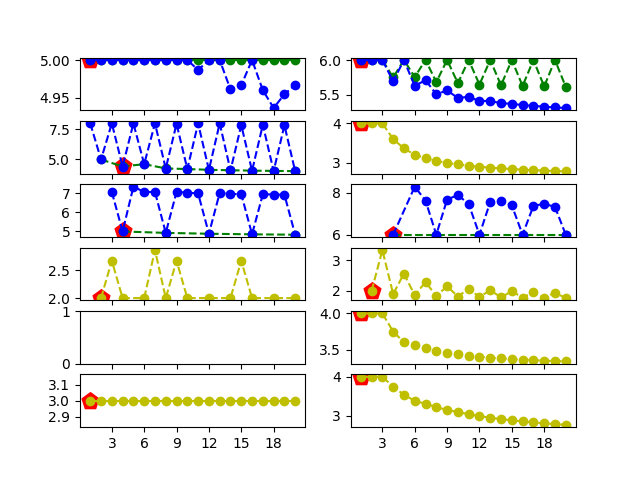
\includegraphics[width=1\textwidth]{fig/iterative.png}
\end{figure}